\documentclass{book}
\usepackage{amsmath, amsfonts,stmaryrd}

\usepackage{xspace}
\usepackage{minted}
\usepackage{url}
\usepackage{tikz}
\usetikzlibrary{positioning,shapes}

\usepackage{mdframed}
\usepackage{xcolor}
\usepackage{pgfplots}
\usepackage{fancyvrb}
\newcounter{Qcours}

\usepackage{graphicx}
\graphicspath{{img}}

\newenvironment{memory}{%
	\noindent
	\VerbatimEnvironment\stepcounter{Qcours}%
	\begin{VerbatimOut}{mem/\theQcours.mem}%
	}{\end{VerbatimOut}%
	\input{|"python memory.py mem \theQcours"}%
}

\newenvironment{commentaire}[1]{%
	\def\FrameCommand{\fboxrule=\FrameRule\fboxsep=\FrameSep \fcolorbox{yellow!50}{yellow!10}}%
	\MakeFramed {\advance\hsize-\width \FrameRestore}
	\noindent {\bf #1}\\
}%
{\endMakeFramed}


\newenvironment{formalisme}[1]{%
	\def\FrameCommand{\fboxrule=\FrameRule\fboxsep=\FrameSep \fcolorbox{red!10}{red!5}}%
	\MakeFramed {\advance\hsize-\width \FrameRestore}
	\noindent {\bf #1}\\
}%
{\endMakeFramed}

\newenvironment{exercice}[1]{%
	\def\FrameCommand{\fboxrule=\FrameRule\fboxsep=\FrameSep \fcolorbox{blue!20}{blue!5}}%
	\MakeFramed {\advance\hsize-\width \FrameRestore}
	\noindent {\bf #1}\\
}%
{\endMakeFramed}

\usepackage{scontents}

\newcommand{\python}{\textsc{python}\xspace}
\newcommand{\C}{\textsc{C}\xspace}
\newcommand{\java}{\textsc{Java}\xspace}
\newcommand{\code}[1]{\texttt{#1}}
\newcommand{\str}[1]{\texttt{\upquote{#1}}}

\newcommand{\eip}{{\tt eip}\xspace}
\newcommand{\rip}{{\tt rip}\xspace}
\newcommand{\eax}{{\tt eax}\xspace}
\newcommand{\ebx}{{\tt ebx}\xspace}
\newcommand{\ecx}{{\tt ecx}\xspace}
\newcommand{\edx}{{\tt edx}\xspace}
\newcommand{\rax}{{\tt rax}\xspace}
\newcommand{\rbx}{{\tt rbx}\xspace}
\newcommand{\rcx}{{\tt rcx}\xspace}
\newcommand{\rdx}{{\tt rdx}\xspace}
\newcommand{\ax}{{\tt ax}\xspace}
\newcommand{\rcs}{{\tt cs}\xspace}
\newcommand{\rds}{{\tt ds}\xspace}
\newcommand{\rfs}{{\tt fs}\xspace}


\newcommand{\hexa}[1]{{\tt 0x#1}}
\newcommand{\bina}[1]{{\tt 0b#1}}

\newcommand{\REG}{{\tt REG}\xspace}
\newcommand{\BYTE}{{\tt BYTE}}
\newcommand{\WORD}{{\tt WORD}}
\newcommand{\DWORD}{{\tt DWORD}}
\newcommand{\QWORD}{{\tt QWORD}}
\newcommand{\vReg}{{\mathfrak{R}}}
\newcommand{\Memory}{{\mathfrak{M}}}


\newcommand{\Addr}{{\mathbf{Addr}}}
\newcommand{\Reg}{{\mathbf{Reg}}}
\newcommand{\Seg}{{\mathbf{Seg}}}

\newcommand{\N}{{\mathbb{N}}}

\newcommand{\Windows}{{\sc windows}}

\newcommand{\Configuration}{{\mathbf{Configuration}}}


\newcommand{\xquatre}{{\tt x86}\xspace}
\newcommand{\sema}[1]{{\llbracket #1 \rrbracket}}

\begin{document}
	
\section*{Une minute d'attention}

Le sujet de ce cours est d'étudier les logiciels malveillants et surtout les techniques que ceux-ci mettent en \oe uvre. Pour bien comprendre ces plaies de l'informatique, il faut prendre le point de vue adverse, mais l'objet du cours reste bien la défense contre les logiciel malveillants. 

L'auteur de ce cours décline toute responsabilité du fait de son emploi à d'autres fins que la défense contre les logiciels malveillants. Rappelons que toute action s'appuyant sur l'emploi d'un logiciel malveillant est punie par la loi. 

D'autre part, je fais l'hypothèse que vous connaissez le langage \C et le langage \python. Je n'utilise pas de constructions très sophistiquées, mais les bases sont requises.

Décrire le fonctionnement complet d'une machine est hors de portée d'un document comme celui ci. Il faudrait une bibliothèque entière pour le faire, et une bibliothèque qui changerait à chaque seconde. Nous ferons  quelques fois des approximations dont l'unique but est de rester simple. Sans quoi, on se noit dans les détails de fonctionnement d'une machine en perdant de vue ce qui est important. L'idée directrice est de donner de quoi raisonner sur le fonctionnement d'un programme, pas de décortiquer le fonctionnement d'un ordinateur. \'Evidemment, comme le programme est exécuté sur l'ordinateur, le fonctionnement de ce dernier ne peut être complètement oublié, mais l'abstraction est le meilleur moyen de pouvoir continuer à travailler.

\medskip
Bonne lecture,

\chapter{Prérequis}

\section{Notations}

Nous utilisons par la suite un certain nombre de notations. Essayons de toutes les grouper ici.

%\'Etant donné deux entiers $a \leq b$, on note $[a, \ldots, b] =\{x \in \ZZ \mid a \leq x \leq b\}$. Et $[a, \ldots, b[ = \{ x \in \ZZ \mid a \leq x < b\}$.

%\'Etant donné deux ensembles $X$, $Y$ et $y \in Y$, on note $\underline{y} : X \to Y$ la fonction $x \in X \mapsto y$. \'Etant donné une fonction $f : X \to Y$, $x \in X$ et $y \in Y$, on note $f[x \mapsto y] : X\to Y $ la fonction définie par
%$$\left\{
%\begin{array}{ll}
%x' \mapsto f(x) & \text{ pour tout } x' \in X \text{ tel que }x' \neq x\\
%x \mapsto y & \text{ sinon}.
%\end{array}\right.$$

%\'Etant donné une fonction $f : X \to Y$, des éléments $x_1, \ldots, x_k \in X$ et $y_1,\ldots, y_k \in Y$, 
%on peut composer les fonctions $f[x_1 \mapsto y_1, x_2 \mapsto y_2, \ldots, x_k \mapsto y_k] = $
%$$\left( (\sigma[x_1 \mapsto y_1])[x_2 \mapsto y_2]\cdots\right)[x_k\mapsto y_k].$$ 

Quand les éléments $x_1, \ldots, x_k$ sont deux à deux distincts, l'ordre importe peu. Par exemple : 
$$f[x_1\mapsto y_1, x_2 \mapsto y_2] = f[x_2\mapsto y_2, x_1 \mapsto y_1].$$

%\begin{formalisme}{Structures de données}
Nous notons pour la suite $\BYTE$ l'ensemble des octets ("byte" en anglais), c'est-à-dire les entiers entre $0$ et $2^8 -1$, $\WORD$ l'ensemble des mots ("word"), les entiers entre $0$ et $2^{16} - 1$,  $\DWORD$ l'ensemble des mots doubles, les entiers entre $0$ et $2^{32} -1$ et  $\QWORD$ l'ensemble des mots quadruples, les entiers entre $0$ et $2^{64} - 1$.
%\end{formalisme}

Etant donné une fonction $M: \QWORD \to \BYTE$, et deux entiers $a \leq b$, on utilise de temps en temps la notation $M[a] = M(a)$ selon qu'on a un penchant d'informaticien ou de mathématicien. \'Etant donnés deux entiers $a \leq b$, $M[a:b] = (M[a], \ldots, M[b-1])$ est la suite des éléments de $M$ entre $a$ et $b$, la suite étant vide si $a=b$. 

On rappelle que dans le modèle little-endian, étant donné $a\in \QWORD$ et $M: \QWORD\to \BYTE$, $$\begin{array}{rcl}
M_2(a) &=& M[a] + M[a] \times 256\\
M_4(a) &=& M[a] + M[a]\times 256 + M[a]\times 256^{2} +M[a]\times 256^{3} \\
M_8(a) &=& \sum_{i = 0}^7 M[a+i] \times {256}^{i}\\
\end{array}$$
désignent respectivement le mot, le mot double, le mot quadruple stocké à l'adresse $a$. Par la suite, quand le contexte est claire, on va oublier les indices $2, 4$ et $8$. 

%On utilise aussi $mem[a:b[ = (mem[a], \ldots, mem[b-1])$, la suite étant vide si $a = b$. 

\begin{commentaire}{Questions/observations}
	Par la suite, vous verrez des blocs en jaune. Ils correspondent à des questions/observations qu'on m'a posées/faites auparavant. 
\end{commentaire}

\begin{formalisme}{Formalisme}
	Les blocs qui sont en rose abordent le problème sous l'angle mathématique/abstrait. Ils sont rédigés à la manière de ce qu'on peut trouver dans un article scientifique. La section notation aurait pu être entièrement en rose. C'eut été un peu lourd.
\end{formalisme}


\chapter{La machine au microscope}

Un ordinateur est l'assemblage de matériels parmi lesquels on trouvera un (ou plusieurs) processeur, des périphériques (claviers, souris, joysticks), de la mémoire (sous diverses formes), un moniteur (qui peut avoir son propre processeur), etc. Au démarrage d'une machine, un premier programme---qualifié de \emph{bootstrap}---met en route le système d'exploitation, lui-même un programme. Le système d'exploitation est en charge d'orchestrer l'utilisation du processeur, une ressource partagée, par l'ensemble des programmes. 

Un ordinateur est donc un système qui peut être vu à plusieurs niveaux~ : on peut partir du "hardware", c'est-à-dire du matériel, on peut prendre le "point de vue" du logiciel d'un utilisateur ou celui du système d'exploitation (OS). \'Evidemment, ces niveaux ne sont pas complètement déconnectés les uns des autres. Dans ce chapitre, nous proposons un modèle de la machine qui rend compte du comportement d'un logiciel exécuté en mode "user", le mode le moins privilégié et le plus commun.

Nous ciblons essentiellement le fonctionnement d'un programme sur un processeur \xquatre en version 64 bits, mais les concepts introduits ont une portée plus large. Pour suivre les exemples, il est conseillé d'utiliser une machine virtuelle pour ceux qui auraient une machine sur une autre architecture, {\sc arm} pour l'exemple. 


\section{Du matériel au virtuel}

Si la machine est un objet physique, carte mémoire, processeurs, caches, souris, etc, elle peut également être vue comme un objet abstrait, mathématique. Cette abstraction est implémentée conjointement par le processeur et par le système d'exploi\-tation. Chacun est conçu pour que l'utilisateur puisse s'appuyer sur cette abstraction. Quand on écrit un programme, on ne s'occupe pas de la tension sur les bus, et c'est bien heureux.

Cette abstraction se révèle extrêmement simple. Notre modèle de machine se réduit à :
\begin{itemize}
	\item de la mémoire virtuelle et
	\item  des registres. 
\end{itemize}

Il y a bien sûr un lien entre les zones de mémoire virtuelle et les caches et autres barrettes physiques de mémoire, mais le programme s'exécute comme s'il \emph{vivait dans le monde virtuel}. Autrement dit, le processeur et l'OS organisent les composants physiques de la machine pour qu'ils apparaissent sous une forme virtuelle auprès des programmes. Pour le programme, l'état de la machine est entièrement décrit par la valeur des registres et la donnée de la mémoire virtuelle. 

Le passage de la mémoire virtuelle à l'architecture physique de la machine va bien au delà de ce polycopié. C'est typiquement l'objet du cours d'architecture. Nous donnerons donc un exposé simplifié du fonctionnement d'une machine. Cette abstraction a un coût: nous ne serons pas en mesure de modéliser des attaques de type {\sc spectre} qui exploitent des effets de cache, voir par exemple \url{https://spectreattack.com}. %Et plus généralement, le modèle est clairement insuffisant pour gérer l'OS lui même ou un driver (c'est-à-dire un programme en mode kernel). 

%Si on fait abstraction du matériel, et si on se place du point de vue d'un programme en cours d'exécution, l'ordinateur est composé d'un bloc de mémoire de grande taille, dite mémoire virtuelle, et d'un petit nombre de 
%mémoires de petite taille (au plus quelques octets),  les \emph{registres}. 

\subsection{Mémoire virtuelle}

La \emph{mémoire virtuelle} est un tableau de cellules mémoires, chacune possédant donc un index appelé \emph{adresse}. Chaque cellule contient un octet. Sur une machine 64 bits, il y a \emph{potentiellement} $2^{64}$ cellules\footnote{Dans les faits,  l'adressage ne peut se faire que sur 48 bits, voire 52 bits, mais nous pouvons faire \emph{comme s'il} était sur 64 bits.}. Ainsi il existe la cellule à l'adresse \code{0}, celle à l'adresse \code{1}, \code{2}, etc. Avec $64$ bits, la limite est donc de $2^{64} \simeq 2 \times 10^{19}$ octets, c'est-à-dire 20Eo (exa octets). Comme ordre de grandeur, selon T. Landauer, la mémoire de l'ensemble de l'humanité serait de l'ordre d'1Eo. Dans les faits, seule une partie de la mémoire est disponible au programme exécuté. Nous y reviendrons en détail.  Un exemple de mémoire virtuelle, la première case contenant la valeur $0xAB$, la dernière $0xEF$. 

\medskip
\begin{memory}
m = Memory(12, 0.6);
m.mark(0, "0")
m.mark(11, "FF\^ {}8")
m.content(0, "AB")
m.content(11, "EF")
m.content(1, "$\ldots$")
\end{memory}

La mémoire est découpée pages, en tranches de 4kO octets (c'est-à-dire par blocs de 0x1000 = 4096 octets). Chacune dispose de droits spécifiques : R, W et X, lecture, écriture et exécution (c.f. le manuel de {\tt mprotect} en \C sous Unix). 

Pour se "promener" dans la mémoire, et voir les droits associés, on pourra utiliser le petit code \C suivant sous Windows, pour avoir les droits à l'adresse 0x1000000 :
\begin{minted}{C}
MEMORY_BASIC_INFORMATION mbi;
VirtualQuery( (void *) 0x1000000, &mbi, sizeof(mbi));
std::cout << mbi.BaseAddress << " " << std::hex << mbi.Protect;
\end{minted}

Une image un peu plus précise de la mémoire est donc :

\medskip
\begin{memory}
m = Memory(12, 0.6);
m.mark(0, "0")
m.mark(11, "FF\^ {}8")
m.content(0, "AB")
m.content(11, "EF")
m.content(1, "$\ldots$")
m.content(3,"01")
m.mark(3, "0x1000")
m.bar(6)
m.content(4, "$\ldots$")
m.add_node((7,0.25), "$\ldots$")
m.bar(9)
m.mark(6, "0x2000")
#BEFORE: \fill[color=red!10] (0,0) -- (3,0) -- (3,0.6) -- (0,0.6) -- cycle;
#BEFORE: \fill[color=blue!10] (3,0) -- (6,0) -- (6,0.6) -- (3,0.6) -- cycle;
#BEFORE: \fill[color=green!10] (9,0) -- (12,0) -- (12,0.6) -- (9,0.6) -- cycle;
\end{memory}
où les couleurs rouge, bleu, vert désignent des droits spécifiques en mémoire. 

\medskip
En plus de ce mécanisme, il y a deux modes d'utilisation du processeur~: le mode "user" et le mode "supervisor" ou "kernel". Dans ce cours, nous travaillons essentiellement en mode "user", c'est le mode de l'utilisateur. Le kernel et les drivers vont agir en mode "supervisor". 

\begin{formalisme}{La mémoire virtuelle}
En termes mathématiques, l'état de la mémoire virtuelle se décrit comme une paire de fonction $(M,\rho)$ où:
\begin{itemize}
	\item $M : \Addr \to \BYTE$ où $\Addr = \QWORD$ pour une machine 64 bits, et $\DWORD$ pour une machine 32 bits.
	\item $\rho: \Addr \to 2^{\{R, W, X\}}$ associe à chaque adresse les droits associés.
	
On note $\frak{V}$ l'ensemble des fonctions $\Addr \to \BYTE$ et $\frak{D}$ l'ensemble des fonctions $\Addr \to 2^{\{R, W, X\}}$. Et enfin, $\Memory = \frak{V} \times \frak{D}$. C'est l'ensemble de toutes les configurations mémoire de notre modèle. 
\end{itemize}

Etant donné un état de la mémoire $M = (m,r) \in \Memory$, on note $M.mem = m$ sa première composante et $M.rights = r$ la seconde. Etant donné $a \in \QWORD$, on se permet d'écrire $M[a]$ pour $M.mem(a)$. Nous reprenons les notations de la Section~\ref{sec:notations}.

La gestion des droits page par page se traduit par l'équation $$\rho(x) = \rho(x)\; \& \; \code{ff\^{}6 f0 00}$$ pour tout $x\in \Addr$. L'hypothèse est implicite par la suite. 	
\end{formalisme}

\subsection{Registres}
Les registres sont des zones de mémoires directement implantées sur le processeur. Les énumérer devient vite fastidieux. Citons quand même ceux qu'on va retrouver régulièrement. 

Les registres courants sont : {\tt rax, rbx, rcx, rdx, rsi, rdi, rsp, rbp, r8, ..., r15, rip, rflags}. Ils font tous 8 octets (64 bits). Ils sont prévus pour contenir des adresses ou des entiers.

Pour les calculs avec les flottants, il y a des registres spécialisés. Ce sont les registres sont {\tt xmm0, ..., xmm7}. Ces registres font 128 bits (et même plus si on prend leur forme {\tt ymmi} (256 bits) ou {\tt zmmi} (512 bits)). 

\begin{commentaire}{Les registres ont une histoire}
Les quatre premiers registres datent des premiers processeurs {\sc intel}, le 8080, dans les années 1970. Ils faisaient au début 8 bits. Et il fallait les combiner pour obtenir des nombres au dessus de 255.
	
Pour des raisons de retro-compatibilité, ces registres sont toujours accessibles aujourd'hui. Par exemple, le registre {\tt ebx} qui date de l'architecture {\tt Intel-386} (32 bits) correspond aux 32 bits de poids faible du registre {\tt rbx}. Le registre {\tt ax} qu'on retrouve sur {\tt Intel-286} correspond aux 16 bits de poids faible de {\tt rax}. Et enfin, {\tt ah} et {\tt al}, tous deux faisant 8 bits correspondent respectivement aux bits de 8 à 16 et aux bits de 0 à 8 du registre {\tt rax}.
	
En résumé, les 8 octets de {\tt rax} s'énumèrent :
	\begin{center}
		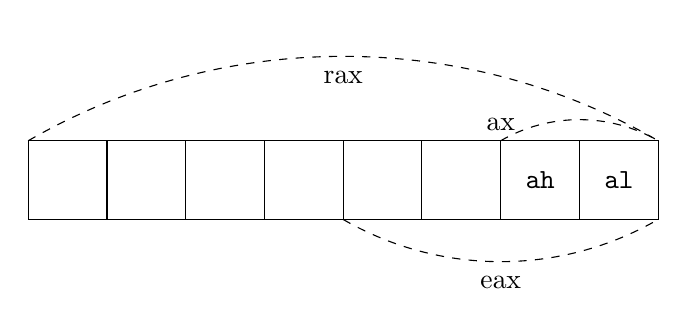
\begin{tikzpicture}
		\draw (0,0) -- (8,0)  -- (8,1) -- (0,1)  --cycle;
		\foreach \i in {1,...,7}{
			\draw (\i,0) -- (\i,1);
		}
		\draw (1,0) -- (1,1);
		\draw (2,0) -- (2,1);
		\draw (3,0) -- (3,1);
		\node (A0) at (6.5,0.5) {\tt ah};
		\node (A0) at (7.5,0.5) {\tt al}; 
		\draw[dashed] (6,1) arc (120:60:2);
		\draw[dashed] (4,0) arc (-120:-60:4);
		\draw[dashed] (0,1) arc (120:60:8);
		\node (Ax) at (6,1.2) {ax};
		\node (Ax) at (6,-0.8) {eax};
		\node (Ax) at (4,1.8) {rax};
		\end{tikzpicture}
	\end{center}
\end{commentaire}

Parmi les registres, il y en a trois qui se distinguent. 
\begin{itemize}
	\item Le registre {\tt rip}, instruction pointer, est le registre qui contient l'adresse de l'instruction à exécuter. 
	\item Le registre {\tt rsp} désigne le "haut de la pile". 
	\item Le registre {\tt rflags} est composé de drapeaux. Le drapeau {\tt ZF} est mis à 1 si quand un calcul arithmétique aboutit à 0. Parmi les autres flags : SF, drapeau du signe (1 quand le nombre est positif, 0 s'il est négatif), CF (carry, 1 si l'opération se termine avec une retenue), OF, (overflow, en cas de dépassement de capacité du registre), PF, (parity). 
\end{itemize} 

Il y a combien de registres en {\sc x86}? Disons une centaine, cela dépend de\ldots la manière de compter. Le registres forment tout un zoo qui est le fruit de l'histoire de cette famille de processeurs. Notons toutefois que la plupart d'entre eux sont spécifiques au mode kernel. Pour celles et ceux qui veulent un aperçu du paysage, je suggère \url{https://blog.yossarian.net/2020/11/30/How-many-registers-does-an-x86-64-cpu-have}.

Quelles sont les propriétés des registres ? Premier point, les registres ont donc des tailles spécifiques. Le registre $\rcs$ est un registre dit de segment. Sa taille est de 2 octets. Les registres ${\tt xmm1}, {\tt xmm2}, \ldots$ vus ci-dessus font 16 octets.

\begin{formalisme}{Modèle des registres}
	Par la suite, on note \REG l'ensemble des registres. Au même titre qu'on a défini la valuation des variables, on peut le faire pour les registres. 
	
	\medskip
	Une \emph{valuation} de registres est une fonction dans $\REG \to \QWORD$. On note $\vReg$ l'ensemble des valuations de registres. 
\end{formalisme}

\begin{commentaire}{Erreur ou imprécision ?}
	Dans la description d'une valuation ci-dessus, le registre {\tt xmm0} qui est dans $\REG$ prend ses valeurs dans $\QWORD$ alors qu'il fait 16 octets (2 $\QWORD$ par conséquent). Comment faire mieux ? 
\end{commentaire}
	
Deuxième point. Les registres permettent de désigner des zones de mémoire. Par défaut, la zone est la valeur du registre. Toutefois, pour les registres de segments, qui ne font deux octets, la zone indiquée est différente. Le registre $\rfs$ par exemple fait référence au mode d'adressage du processeur (via des tables accessibles en mode kernel). La valeur donnée par $\rfs$ ne correspond pas à la valeur du registre mais au contenu indexé dans une table. Faisons abstraction de ce mécanisme, nous \emph{ferons comme si} le registre désignait une valeur arbitraire en mémoire.

\begin{minted}{c}
unsigned short fs;
asm("mov %%fs, %0" : "=r"(fs));
uint64_t at_fs;
asm ("lea %%fs:(0), %0" : "=r"(at_fs));
printf("fs=%x: fs points to: %lx\n", fs, at_fs);
\end{minted}

%Pour résumer, nous notons $\Reg$ l'ensemble des registres. Pour chaque registre $r\in \Reg$, $|r|$ désigne la taille du registre en nombre d'octets et $[r]$ l'index qu'il désigne en mémoire virtuelle. L'état des registres se décrit alors comme une fonction $R$ qui a chaque registre associe $R(r) \in [0\ldots 256^{|r|}]$ sa valeur et $r \mapsto [r]$ est la fonction d'adressage.  

Etant donné $M \in \Memory$ un état de la mémoire virtuelle et $R$ l'état des registres. La notation $M[r] = M.mem(R(r))$ désigne l'octet contenu à l'adresse indiquée par un registre $r \in \Reg$.% Par la suite, nous utiliserons la version simplifiée: $M[r]$. 

%Nous revenons sur certains registres en section~\ref{sec:asm}. 

\subsection{Instructions}

\newcommand{\Instr}{{\tt Instr}}

Jusque là, nous avons décrit l'état d'une machine. Attaquons nous maintenant au calcul. Les instructions machines sont les plus petits éléments qui le pilote.

\begin{formalisme}{Instruction}
Une instruction est une suite d'octets associée à une sémantique (qui spécifie ce que fait l'instruction). 
	
L'ensemble des instructions, noté $\Instr$, a la propriété d'être préfixe. C'est à dire qu'il n'y a pas deux instructions dont l'une est le début de l'autre.  	
\end{formalisme}
Voici un 6 instructions machine : 
\begin{minted}{asm}
90
55
89, B8
B8, 01, 02, 03, 04
67, 48, 8B, 41, 0C
FF D0
C3
\end{minted}

On peut maintenant résumer le fonctionnement d'une machine.  L'exécution d'un programme procède de la manière suivante. A chaque étape, le processeur lit les cases mémoires $M[\rip], M[\rip+1], M[\rip+2], \ldots$ Trois possibilités :  soit un préfixe\footnote{début de la suite.} de la suite correspond à une instruction machine  et la zone lue a les droits en lectuRe et en eXecution, auquel cas l'instruction est exécutée. Soit il y a un problème de droit ou bien encore la suite ne correspond pas à une instruction, dans ce cas un mécanisme d'exception prend en charge l'erreur. 

Ainsi, si la valeur de  $M[\rip]$ est $\hexa{90}$, le processeur reconnaît l'instruction machine \code{nop} qui consiste à ne rien faire\footnote{En fait, elle incrémente tout de même la valeur de \rip\ de $1$. }. Si la suite commence par : \code{48,83,C0, 09},  il s'agit de l'instruction qui rajoute $9$ au registre \rax\ et passe à l'instruction suivante\footnote{C'est-à-dire incrémente \rip de $4$.}.  

Le programme  poursuit son exécution tant qu'une \emph{interruption} ne se produit pas. Les interruptions (en règle générale externes au programme en cours) peuvent apparaître à diverses occasions, une instruction illégale comme nous avons vu plus haut, une modification au niveau matériel ou bien la frappe d'une touche clavier. Suite à l'interruption, et selon une certaine politique de priorité, le système d'exploitation "reprend" la main, en d'autres termes, la valeur de \rip est modifiée directement par le processeur, en dehors du contrôle du programme. Le système rendra éventuellement la main au programme plus tard. 

\begin{formalisme}{Exécution}
\'Etant donné une configuration $C = (M, R) \in \Memory \times \vReg$, la machine va lire la suite d'octets à partir de $\rip$. Trois cas : 
\begin{itemize}
	\item Lors de la lecture, il y a une adresse $x$ pour laquelle $X \not\in M.rights[x]$. Une exception est envoyée au système. 
	\item La suite d'octets ne correspond pas à une instruction. Dans ce cas, une exception est également levée. 
	\item Sinon, l'instruction est exécutée. Ce qui a pour effet de modifier la configuration. La modification étant spécifiée par l'instruction elle même.
\end{itemize}
\end{formalisme}

Travailler directement avec des instructions machines peut vite être un exercice de mémoire fastidieux. Nous allons plutôt utiliser une représentation en assembleur de celles-ci. Pour les instructions précédentes : 
%Il y a plusieurs manières de les voir. De manière abstraite, c'est un ensemble qu'on peut lister : 
\begin{minted}{asm}
nop
push rbp
add rax, rbx
mov rax, 0x04030201
mov rax, qword ptr[rcx+12]
call rax
ret
\end{minted}

La correspondance entre le code assembleur et le code machine peut se retrouver sur un site comme : \url{https://defuse.ca/online-x86-assembler.htm}. 

La liste des instructions se trouve dans le(s) manuel(s) du(es) constructeur(s) du processeur. Par exemple, on retrouvera pour INTEL/x86\_64 les instructions à \cite{IntelSetInstruction}. Attention, l'ensemble des instructions varie au cours du temps, certaines apparaissent, d'autres disparaissent. Par la suite, on note $\Instr$ l'ensemble des instructions. 

\begin{commentaire}{Quelques mots sur l'encodage et la structure des instructions}
Une \textit{instruction} se décompose selon le format\footnote{Plus de détails à \url{http://ref.x86asm.net/coder32.html} par exemple.} :%TODO dire qu'en bytes bah c'est quasiment arei
\begin{eqnarray*}
	\Instr& ::=& \code{prefix}_1 \dots \code{prefix}_k \; \code{opcode} \; \code{Arg}_1 \dots \code{Arg}_\ell\\
	\code{Arg} &::=& \code{Imm}\ |\ \Reg\ |\ \code{Mem}\\
	\label{eq3} \code{Mem} &::=& (\Seg[\Reg_1+scale*\Reg_2+\code{Disp}], size)\\ 
	\code{prefix} &:::=& {\tt rep}, {\tt lock}, {\tt data16}, \ldots\\
	\code{opcode} &::=& {\tt add}, {\tt jmp}, {\tt call}, \ldots \\
	\Seg & ::=& {\tt cs}, {\tt ds}, {\tt es}, \ldots \\
	\Reg & ::=& {\tt rax}, {\tt ebx}, \ldots
\end{eqnarray*}
où \code{Imm}, \code{Disp} désignent un immédiat (un nombre), $scale\in\{1,2,4,8\}$ et $size\in\{1, 2, 4, 8\}$. 

Le codage de l'instruction suit la structure ci-dessus : chaque préfixe est stocké sur un octet. L'opcode désigne l'opération à réaliser. Il est stocké sur un, deux ou trois octets. Ensuite, pour les arguments, les immédiats sont codés tels qu'ils apparaissent en mémoire. Les registres, registres de segments, scale et size et les références en mémoire ont un mécanisme spécifique (voir le codage \code{mod/rm}+sib). Un exemple, l'instruction $$\code{data16 adc [rbx+rcx*4+0x12],0x1357}$$
est encodée \code{66,81,54,8B,12,57,12}: 

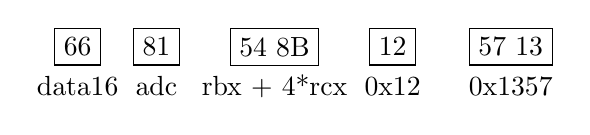
\begin{tikzpicture}
\node[draw,shape=rectangle] (A) at (0,0) {66};
\node (Aa) at (0,-0.5) {data16};
\node[draw,shape=rectangle] (B) at (1,0) {81};
\node (Ba) at (1,-0.5) {adc};
\node[draw,shape=rectangle] (C) at (2.5,0) {54 8B};
\node (Ca) at (2.5,-0.5) {rbx + 4*rcx};
\node[draw,shape=rectangle] (D) at (4,0) {12};
\node (Da) at (4,-0.5) {0x12};
\node[draw,shape=rectangle] (E) at (5.5,0) {57 13};
\node (Ea) at (5.5,-0.5) {0x1357};
\end{tikzpicture}
\end{commentaire}


%L'encodage d'une instruction est injectif (dans les suites d'octets). A une instruction correspond un unique encodage. Par la suite, nous ne distinguons plus une instruction de son encodage.
%Enfin, c'est un encodage dit préfixe :  l'encodage est tel qu'il n'y a pas deux instructions différentes dont l'encodage de l'une soit préfixe de l'autre. 

%\subsection{En résumé}

%L'état de la machine est donc décrite par la mémoire virtuelle et les registres. En termes mathématique, il s'agit d'un triplet $(M, \rho, R)$ désignant respectivement la valeur de chaque cellule en mémoire, les droits associés et la valeur des registres. Un tel triplet s'appelle une configuration et on note $$\Configuration = (\Addr \to \BYTE) \times (\Addr \to 2^{\{R,W,X\}}) \times (\Reg \to \BYTE^A)$$ 
%l'ensemble de toutes les configurations. Enfin, étant donnée une configuration $C$, $M_C$ désigne la valuation de sa mémoire, $\rho_C$ ses droits et $R_C$ la valuation de ses  registres. 


%Selon l'usage, on peut "oublier" les droits en mémoire. On obtient alors un modèle moins précis mais plus simple. S'il est suffisant pour rendre compte du phénomène envisagé, il n'y a pas de raisons de se compliquer la vie. Au contraire, si on s'intéresse à l'attaque {\sc spectre}, le modèle avec valeur et droits n'est pas assez précis. Dans ce cas, il faudra rajouter des informations concernant le(s) cache. Pareil, si on doit tenir compte de l'OS--par exemple les appels systèmes, le modèle sera insuffisant. 

%Tout l'art consiste à trouver le bon niveau d'abstraction.

%\section{Une sémantique opérationnelle}

%Les  processeurs modernes de l'architecture {\sc x86} reconnaissent plus d'un millier d'instructions différentes. On ne les décrira pas ici. Toutefois, on pourra observer que chaque instruction lit et modifie un ou plusieurs registres, éventuellement 1, 2, 4 ou 8 octets en mémoire\footnote{\`A l'exception de certaines instructions de manipulation de chaînes comme {\tt rep stosb} qui modifient un nombre arbitraires d'octets, mais ce type d'instruction prend autant de cycles machine.}.  Il n'y a, d'une certaine manière, que huit types de données : 
%\begin{itemize}
%	\item 1 octet = {\tt byte}, 
%	\item 2 octets = {\tt word},
%	\item 4 octets = {\tt dword},
%	\item 8 octets = {\tt qword},
%	\item 10 octets = {\tt tword} pour les flottants en précision étendue,
%	\item 16 octets = {\tt oword}, 32 = {\tt yword} et 64 {\tt zword} pour les registres spécifiques correspondant : {\tt xmm}, {\tt ymm} et {\tt zmm}
%\end{itemize}

%Les autres structures de données du \C, tableaux, listes, chaînes de caractères, etc sont définies à l'aide de ces briques de base.

%Les instructions machine "en font le moins possible". Par exemple, pour une multiplication, il n'y a pas de vérification du type des éléments manipulés, entiers signés ou non, flottants, ni sur la taille: octet, mot, mot double ou quadruple. La machine autorise l'application  de la multiplication des flottants à un octet signé et à un mot non signé.  En d'autres termes, le programmeur doit gérer le type de chaque zone mémoire.

%En conclusion, le code machine, c'est la politique des nombreux petits pas sans filets.  Les langages de plus haut niveau comme \C ou \python permettent de structurer à plus grande échelle les programmes, ils nous rapprochent de la vue algorithmique.  Pour cela, ils nous offrent essentiellement des structures de contrôle de haut niveau, un plus large éventail de données avec un typage et les outils pour les manipuler. 

%\subsection{Sémantique des instructions}
%
%Quel modèle mathématique rend compte du comportement de la machine. Ma\-thé\-matiquement, on fait l'hypothèse que l'on dispose d'une fonction $${\bf step} : \Configuration \to \Configuration$$
%qui exécute une étape de calcul, c'est-à-dire une instruction machine. Cette fonction peut être décrite par la sémantique de chaque instruction séparément. Etant donnée une instruction $I$, on note 
%$$\sema{I}(M,\rho, R)$$ la configuration obtenue après application de l'instruction $I$ sur la configuration $(M,\rho,R)$. 
%
%Par conséquent, pour une configuration $C = (M,\rho, R)$,  
%$${\bf step}(M,\rho,R) = \sema{I}(M,\rho,R)$$ 
%où $I$ est l'instruction à l'adresse $R(\rip)$, par la suite simplifié sous la forme $\rip$ quand le contexte est clair.
%
%
%En outre, autre hypothèse usuelle, la mémoire n'est modifiée qu'en un nombre borné de position. En d'autres termes, il existe $Mmax > 0$ tel que pour toute configuration $C$, $|\{x \in \Addr : M_{{\bf step}(C)}[x] \neq M_C[x] \}| \leq Mmax$ où $|X|$ désigne le cardinal de l'ensemble $X$.
%
%
%\section{L'assembleur pour les nuls}\label{sec:asm}
%
%Faisons un tour d'horizon de l'assembleur X86. 
%
%\subsection{Registres}
%Petit tour (incomplet) des registres. Les registres se classent en plusieurs catégories, les registres généraux sont 
%$$\tt rax, rbx, rcx, rdx, rsi, rdi, r8, r9, \ldots, r15$$
%ils servent à tout et à rien de particulier. Les registres $\tt rsi$ et $\tt rdi$ servent pour les instructions manipulant des chaînes de caractères. Le "s" de $\tt rsi$ vient de "source", le "d" de $\tt rdi$ pour "destination". 
%Les registres
%$$\tt rbp, rsp$$
%sont le "base pointer" et le "stack pointer". Le registre $\tt rsp$ donne la position courante sur la pile. Le registre $\tt rbp$ donne la position en mémoire des arguments de la fonction courante. Attention, l'emploi de ces registres est conventionnel\footnote{Chercher "Application Binary Interface" sur le web.}. 
%Le registre
%$$\tt rip$$
%désigne l'instruction courante. Le registre 
%$$\tt rflags$$
%contient l'état des flags. Les flags sont mis à jour pour indiquer des informations sur le calcul. Le bit 0 de $\tt rflags$ qui s'appelle $\tt cf$ pour "carry flag" indique que la dernière opération s'est terminée par une retenue (carry). Deux autres exemples de flags  : bit 6, $\tt zf$ (zero), bit 7, $\tt sf$ (signe). 
%
%Enfin, on rencontrera les registres de segments : 
%$$\tt cs, ds, ed, fs, gs, ss$$
%qui ont eu une fonction importante dans le contexte des machines à addressage sur 16 bits (cs: "code segment", ds : "data segment", ss : "stack segment", etc). Ils ne sont plus employés à l'exception de {\tt fs} et {\tt gs} que nous reverrons plus tard. Ces registres sont utilisés par l'OS pour désigner des zones de mémoire pour la gestion des processus. 
%

\chapter{Rappels en C et assembleur}

Ce chapitre n'est pas un cours de C, mais des rappels de ce qui sera utilisé par la suite. 

\section{Manipulations de pointeurs, formats, et joyeusetés}

Quelques lignes à connaître par c\oe ur. 

\begin{minted}[linenos]{C}
int _tmain(int argc, _TCHAR* argv[]){
int i = 0x12345678, j = 32;
printf("[%p] = %d, [%p] = %d \n", &i, i, &j, j );
char *p = (char *) & i;
for(int k = 0 ; k < 4 ; ++k) printf("%02x ", p[k] & 0xff);
uint32_t a = (uint32_t) &i;
int *k = (int *) a;
k--;
printf("k = [%p], p = [%p]\n", k);
*k += 3;//k[0] = 3;
printf("%d\n", j);
\end{minted}

Dont voici le résultat sur la console : 

\begin{minted}{C}
[0012FF78] = 305419896, [0012FF74] = 32
78 56 34 12 
k = [0012FF74], p = [0012FF77]
35
\end{minted}

Quelques commentaires. 

\begin{itemize}
	\item Ligne 2 : deux déclarations de variables.
	\item Ligne 3 : affichage des pointeurs "\%p", notation "\&p" pour désigner l'adresse ou la variable est stockée. 
	\item Ligne 4 : une conversion de type. Les pointeurs sont des nombres. 
	\item Ligne 5 : le phénomène little-endian. Note : dans \code{"\%02x", p[k] \& 0xff}, le format attend un entier sur 4 octets, or \code{p[k]} n'en fait que 1.
	\item Ligne 7/8/9 : attention à l'arithmétique des pointeurs !
	\item Ligne 10 : un effet de bord. L'"erreur" de la ligne 8 conduit à la modification de la valeur de \code{j}\footnote{Attention, cet effet est fonction du compilateur !}
\end{itemize}

\section{Fonctions}

Un programme en C est une liste de déclarations. Parmi celles-ci, il y a les déclarations de variables et les déclarations de fonctions. Le code C une fois compilé garde cette structure globale : les variables globales d'un côté, les fonctions de l'autre. 

Un pointeur de fonction désigne la première instruction de la fonction. Voici un petit exemple d'emploi d'un pointeur de fonction (les déclarations initiales sont omises) : 

\begin{minted}[linenos]{C}
typedef int (*fun_float_int_to_int)(float,int);
int trunc_prod(float r, int i){ return (int) (r * i); }
...
fun_float_int_to_int f = trunc_prod;
printf("%d", f(3.14f, 4));
\end{minted}

Quelques commentaires : 

\begin{itemize}
	\item Ligne 1 : déclaration du type des fonctions, 
	\item Ligne 4 : déclaration d'une variable "fonction",
	\item Ligne 5 : appel de la fonction via la variable. 
\end{itemize}

\paragraph{Décoration sur les déclarations de fonctions }

Deux décoration utilisées de temps en temps. 

\begin{minted}[]{C}
__declspec(noinline) int f(float r){...} //ne doit pas être inlinée
__declspec(naked) void f(){...}    //compilée sans sauvegarde de ebp
\end{minted}

La première évite que la fonction "disparaisse" du fait de la compilation. Pour la seconde, le compilateur ne rajoutera pas la mise en place du frame de la fonction. 



\section{Assembleur}

\subsection{Instructions}
Commençons par les affectations. Voici un certain nombre d'instructions :  
\begin{minted}{asm}
mov rax, 0x1234     ; rax = 0x1234
mov rbx, rax        ; rbx = rax
mov rbx, [0x1234]   ; rbx = *((qword *) 0x1234)
mov ebx, [0x1234]   ; ebx = *((dword *) 0x1234) 
mov ebx, dword ptr[0x1234] ; autre forme de l'instruction précédente
mov bx, [0x1234]    ; bx = *((word *) 0x1234 )
mov bl, [0x1234]    ; bl = *((byte *) 0x1234)
mov rbx, [rax]      ; rbx = *((dword *) rax)
mov rbx, [rax+4*rcx+0x12] ; rbx = *((dword *) rax+0x12) or rbx = rax[0x12]
mov rbx, fs:[0x30]  ; rbx = [fs+0x30]
lea rax, [rbx+4*rcx+0x12] ; rax = rbx + 4*rcx + 0x12
\end{minted}

Quelques opérations arithmétiques : 
\begin{minted}{asm}
xor eax, eax    ; eax ^= eax or eax = 0
add rax, rbx    ;  rax += rbx
sub rax, 0x12   ; rax -= 0x12
imul rax, [rbx] ; signed mul, rax *= [0x12] seen as qword 
imul rbx        ; rax *= rbx (rax is implicit) 
mul rbx         ; unsigned mul, rax *= rbx 
fmul [rsp+8]    ; floating point multiplication (st(0) is implicit)
idiv  [0x1234]  ; ah = rax / *(0x1234), al = rax % *(0x1234)
\end{minted}
Ces opérations vont mettre à jour le registre des flags (carries, zero, etc). Mise à jour des flags,
\begin{minted}{asm}
cmp rax, rbx    ; ZF == (rax - rbx == 0), SF == (rax - rbx > 0)
cmp rax, 0x12   ; 
test rax, rbx   ; ZF == (rax & rbx == 0)
\end{minted}


Opérations sur la pile : 
\begin{minted}{asm}
push eax        ; empilement
pop rbx         ; dépilement
push 0x12       ; empilement de 8 octets (avec des zeros)
pushf           ; "push rflags"
popf            ; "pop rflags"  
\end{minted}

Instructions de contrôle (où next\_ins désigne l'adresse de l'insruction suivante) : 
\begin{minted}{asm}
jmp 0x1234      ; rip = 0x1234 <=> goto 0x1234
jmp [0x1234]    ; rip = [0x1234]
jmp rax         ; rip = rax
jmp [rax]       ; rip = *rax
jz 0x1234       ; si ZF rip = 0x1234 sinon rip = next_ins
; jnz (not zero), jle (lower or equal), jg (greater), etc
\end{minted}

Appels de fonctions
\begin{minted}{asm}
call 0x1234 ; push next_ins; rip = 0x1234
ret         ; pop rip
call rbx
call [rax+0x12]
call [0x1234]
leave       ; rsp = rbp, pop rbp
\end{minted}

Interruptions
\begin{minted}{asm}
int3        ; interruption, utilisée par le debugger
\end{minted}

\chapter{De la machine au programme}

Lorsqu'on double-clique sur un programme, il est exécuté. Le système d'exploitation va mettre en place une mémoire virtuelle, charger les bibliothèques, initialiser les registres, en d'autres termes, préparer la configuration initiale du programme. Dans ce chapitre, on va voir ce qui se passe plus en détails. 

\section{Le programme en mémoire}

Dans un premier temps, observons la structure de la mémoire au démarrage du programme. Les expériences sont présentées en \C sous Windows. Pour Linux, il y a pleins de variations, mais on retrouve assez rapidement les analogies. Compilons le programme suivant (cf. github::basics/starting.c) : 

\begin{minted}[linenos]{C}
#include "stdafx.h"
#include <stdlib.h>
char a ='A',b='B';
int _tmain(int argc, char *argv[]){
	int i = 42, j;
	int *p =(int *) malloc(sizeof(int));
	printf("[%p] = %d\n", &i, i);
	printf("[%p] = %c\n", &a, a);
	printf("[%p] = %x\n", p, *p);
	printf("_tmain = %p\n", _tmain);
	printf("printf = %p\n", printf);
	return 0;
}
\end{minted}

Ce programme montre les quatre grandes zones de mémoire visibles (avec un des droits R, W, X) à l'utilisateur :  le programme lui-même, la pile, le tas, et la zone des bibliothèques partagées. Plus en détail : 
\begin{itemize}
	\item La pile contient typiquement : les variables locales des fonctions (\code{i, j}), les retours des fonctions. On retrouve donc une adresse dans la pile à la ligne 7. 
	\item Le tas contient toutes les données allouées dynamiquement, typiquement avec la fonction \code{malloc}, ligne 9.  
	\item   Le programme va contenir les instructions (\code{main}, ligne 10), les variables globales (\code{a},\code{b}, ligne 8), et différentes ressources (icones, etc). 
	\item  Enfin, les DLLs ont la même structure que l'exécutable lui-même (\code{msvcr.dll} qui contient le code de \code{printf}, ligne 11). Elles vont avoir leur propre pile, leur propre tas, etc. 
\end{itemize}

En résumé, 

\medskip
\begin{memory}
m = Memory(12, 0.6)
m.zone(6,8,"red!10")
m.mark(6,"EXE")
m.content(6,"$\code{4D}\ldots$")
m.zone(1,2,"yellow!20")
m.mark(1.5, "STACK")
m.zone(3.5,5,"green!20")
m.mark(4.2, "HEAP")
m.zone(9,10,"blue!20")
m.mark(9.5, "KERNEL32.dll")
m.zone(10.5,11.5,"blue!20")
m.mark(10.9, "MSVCR100.dll",1)
m.content(1.15,"\code{RWX}",0)
m.content(3.8,"\code{RWX}",0)
m.mark(1.5, "\&i:12FF74", 0.5, 1)
m.mark(4.2, "p:304018", 0.5, 1)
m.mark(6.6, "\_tmain:401000", 0.5, 1)
m.mark(7.2, "\&a:403018",1,0)
m.mark(11, "printf:78B056B4", 0.5, 1)
m.bar(1,2,8,3.5,5,9,10,10.5,11.5)
\end{memory}

Si on fait un zoom sur le programme lui-même, on obtient la structure suivante (avec une compilation standard sous VisualC) : 

\bigskip
\begin{memory}
m = Memory(12, 0.6)
m.zone(2,11,"red!10")
m.bar(2,3.5,5,6.5,8,9.5,11)
m.mark(2.8, "header")
m.mark(4.3, ".text")
m.mark(5.7,".rdata")
m.mark(7.2,".data")
m.mark(8.8,".reloc")
m.mark(10.2,".rsrc")
m.mark(2,"\code{400000}",0.5,1)
m.mark(3.5,"\code{401000}",0.5,1)
m.mark(5,"\code{402000}",0.5,1)
m.mark(6.5,"\code{403000}",0.5,1)
m.mark(8,"\code{404000}",0.5,1)
m.mark(9.5,"\code{405000}",0.5,1)
m.mark(11,"\code{406000}",0.5,1)
m.content(2.5,"\code{RX}",0)
m.content(4,"\code{RX}",0)
m.content(5.5,"\code{R}",0)
m.content(6.8,"\code{RW}",0)
m.content(8.5,"\code{RW}",0)
m.content(10,"\code{R}",0)
m.content(11.1, "\ldots", 0)
m.content(1,"\ldots", 0)
\end{memory}

Le header du programme spécifie l'adresse de base, \code{400000}, le nom, la position relative, la taille, les droits en mémoire associé à chacune des sections :\code{.text, .rdata}, etc. Il spécifie également les DLL importées, la taille de la pile demandée ainsi que la taille du tas. Voir la Section~\ref{sec:pe} sur la structure du PE pour plus de détails. 


\section{Promenade dans le PE}

Une section écrite d'après : 
\begin{itemize}
	\item \url{https://learn.microsoft.com/en-us/previous-versions/ms809762(v=msdn.10)}
\end{itemize}

Un fichier exécutable \Windows\ contient : 
\begin{itemize}
	\item une partie \code{DOS},
	\item un \code{header} pour la partie \code{PE}
	\item et une liste de sections.
\end{itemize} 

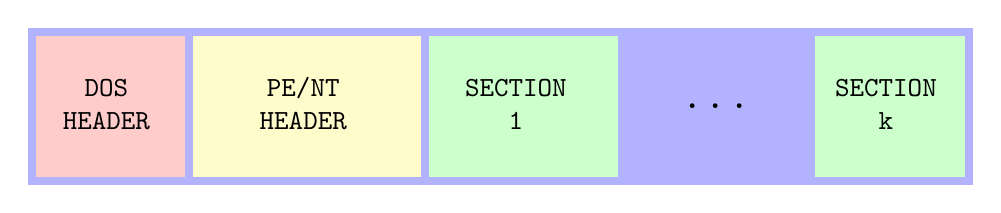
\begin{tikzpicture}
\fill[blue!30] (0,0) -- (12,0) -- (12,2) -- (0,2) -- cycle;
\fill[red!20] (0.1,0.1) -- (2,0.1) -- (2,1.9) -- (0.1,1.9) -- cycle;
\fill[yellow!20] (2.1,0.1) -- (5,0.1) -- (5,1.9) -- (2.1,1.9) -- cycle;
\fill[green!20] (5.1,0.1) -- (7.5,0.1) -- (7.5,1.9) -- (5.1,1.9) -- cycle;
\fill[green!20] (10,0.1) -- (11.9,0.1) -- (11.9,1.9) -- (10,1.9) -- cycle;
\node at (1,1) {\begin{tabular}{c}\code{DOS}\\ \code{HEADER}\end{tabular}};
\node at (3.5,1) {\begin{tabular}{c}\code{PE/NT}\\ \code{HEADER}\end{tabular}};
\node at (6.2,1) {\begin{tabular}{c}\code{SECTION}\\ \code{1}\end{tabular}};
\node at (10.9,1) {\begin{tabular}{c}\code{SECTION}\\ \code{k}\end{tabular}};
\node at (8.8,1) {\huge \ldots};
%\node (A) at(0,0) {\includegraphics[width=7cm]{img/pe_basic_structure.png}};
%\node (B)[right=10mm of A] {\includegraphics[width=7cm]{img/kaitai_view_on_pe.png}};
\end{tikzpicture}


\medskip
Voici un extrait d'un exécutable vu sous \url{https://ide.kaitai.io} : 

\medskip
\noindent
\begin{tikzpicture}
\node (A) at(0,0) {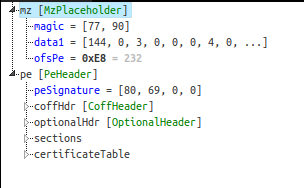
\includegraphics[width=7cm]{img/pe_basic_structure.png}};
\node (B)[below right=-46mm and 2mm of A] {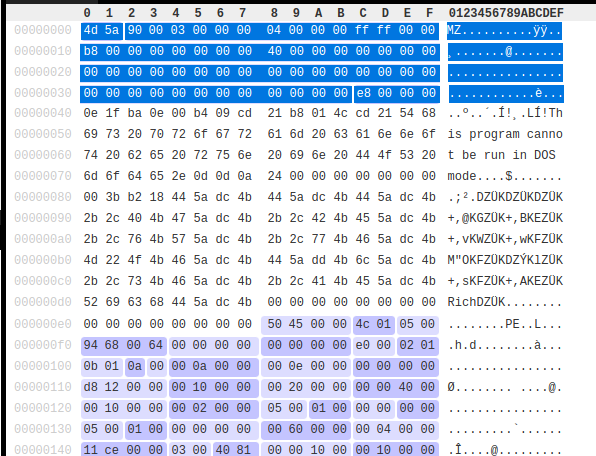
\includegraphics[width=7cm]{img/kaitai_view_on_pe.png}};
\end{tikzpicture}

%Le format des exécutables modernes de \Windows\ est le format PE, lui-même une extension du format DOS (celui des années 80). En quelques lignes, 

\begin{itemize}
	\item La première partie est la partie DOS. Ells suit une structure qui s'appelle \code{IMAGE\_DOS\_HEADER}, accessible dans \code{"Windows.h"}. Elle commence par le 'magic number' \code{4d 5a}, \code{MZ} en \code{ascii}, "MZ" étant les initiales de Mark Zbikowski, un des développeurs de DOS.  A l'octet \code{3c}, on trouve la position du point d'entrée de la structure propre au format PE (Portable Executable).
	\item La partie \code{PE} commence par "PE" en \code{ascii}, \code{50 45}. Elle suit la structure \code{\_IMAGE\_NT\_HEADERS} dont on reparlera plus en détail ci-dessous.
	\item Chaque section de l'exécutable est spécifiée dans l'\code{OptionalHeader}. Elles apparaîssent en séquence après le header \code{\_IMAGE\_NT\_HEADERS}. 
	%\item Enfin, le code se clôt avec un certificat.  
\end{itemize}

La partie \code{PE} est spécifiée comme suit : %commence par \code{PE} en \code{ascii}, \code{50 45}. Elle suit la structure 
\begin{minted}{C}
typedef struct _IMAGE_NT_HEADERS {
  DWORD                   Signature;	//magic=50 45 00 00
  IMAGE_FILE_HEADER       FileHeader;	
  IMAGE_OPTIONAL_HEADER32 OptionalHeader;
} IMAGE_NT_HEADERS32;
\end{minted} 

%La signature est la suite de caractères \code{50 45 00 00}.
 La structure \code{FileHeader} contient les informations suivantes : 

\begin{minted}{C}
typedef struct _IMAGE_FILE_HEADER {
  WORD  Machine;		//indique si on est sur 32 ou 64 bits
  WORD  NumberOfSections;       //nombre de sectiosn
  DWORD TimeDateStamp; /
  DWORD PointerToSymbolTable;   //servait pour le debugger
  DWORD NumberOfSymbols;        //pareil
  WORD  SizeOfOptionalHeader;
  WORD  Characteristics;        // le type de fichier : DLL, EXE, etc
} IMAGE_FILE_HEADER,
\end{minted}

La partie \code{OptionalHeader} contient toutes les informations nécessaires au chargement du programme en mémoire, et en particulier la celles concernant les sections. 

\begin{minted}{C}
typedef struct _IMAGE_OPTIONAL_HEADER {
WORD                 Magic;		    //is it 32 or 64 bits ?
BYTE                 MajorLinkerVersion;
BYTE                 MinorLinkerVersion;
DWORD                SizeOfCode;	   	//size of X pages
DWORD                SizeOfInitializedData;
DWORD                SizeOfUninitializedData;
DWORD                AddressOfEntryPoint;
DWORD                BaseOfCode;
DWORD                BaseOfData;
DWORD                ImageBase;
DWORD                SectionAlignment;    	//usually 0x1000
DWORD                FileAlignment;
WORD                 MajorOperatingSystemVersion;
WORD                 MinorOperatingSystemVersion;
WORD                 MajorImageVersion;
WORD                 MinorImageVersion;
WORD                 MajorSubsystemVersion;
WORD                 MinorSubsystemVersion;
DWORD                Win32VersionValue;		    //must be 0
DWORD                SizeOfImage;  	//size of the exe in memory
DWORD                SizeOfHeaders;
DWORD                CheckSum;	  	//checksum of the file
WORD                 Subsystem;
WORD                 DllCharacteristics;	 //info for DLLs
DWORD                SizeOfStackReserve;	 //stack size required
DWORD                SizeOfStackCommit;  	//"initialized" stack
DWORD                SizeOfHeapReserve;     		//for heap
DWORD                SizeOfHeapCommit;
DWORD                LoaderFlags;			//deprecated
DWORD                NumberOfRvaAndSizes; //number of directory_entries
IMAGE_DATA_DIRECTORY DataDirectory[IMAGE_NUMBEROF_DIRECTORY_ENTRIES];
} IMAGE_OPTIONAL_HEADER32
\end{minted}

Arrivent les \code{IMAGE\_DATA\_DIRECTORY}. Ce sont des tables/des structures  qui contiennent des informations complémentaires (listées ici par ordre d'importance). Chaque entrée a le type : 

\begin{minted}{C}
typedef struct _IMAGE_DATA_DIRECTORY {
  DWORD VirtualAddress;
  DWORD Size;
} IMAGE_DATA_DIRECTORY
\end{minted}
qui donne la position relative de la structure en mémoire et sa taille. Il y a 16 structures/tables (listées ici par ordre d'importance) :  

\bigskip
\begin{tabular}{| l | l |}
	\hline
Value	&Meaning \\
\hline
0 & Export directory\\
12&Import address table\\
1&Import directory \\
5 &Base relocation table\\
9 & Thread local storage directory\\
7 &Architecture-specific data \\
11&Bound import directory\\
14&COM descriptor table\\
6&Debug directory\\
13&Delay import table\\
3 &Exception directory \\
8 & The relative virtual address of global pointer\\
10 &Load configuration directory\\
2 & Resource directory \\
4& Security directory \\
\hline
\end{tabular}


\begin{commentaire}{En bref}
La table EAT (Export Address Table) contient une structure liant : un nom de fonction, son ordinal et sa position relative dans l'exécutable. Au chargement d'une bibliothèque partagée par un exécutable $E$, l'OS lit cette table pour retrouver les adresses des fonctions appelées par $E$.



La table IAT (Import Address Table) contient une structure liant le nom des fonctions importées et les addresses correspondantes. Après avoir retrouvé les addresses des fonctions dans la table d'export de la bibliothèque associée, l'OS remplit la table des adresses.  
\end{commentaire}

\subsection{Reconstruire l'exécutable à partir de l'adresse de base}

Pour modéliser l'exécutable, nous allons employer la structure suivante : 

\begin{minted}{C}
typedef struct{
	PIMAGE_DOS_HEADER     dos_header;
	PIMAGE_NT_HEADERS   nt_header;
	PIMAGE_SECTION_HEADER sections;
} pefile32_t;

int parse_pe_in_mem(void *p, pefile32_t & pe){
	pe.dos_header = (PIMAGE_DOS_HEADER) p;
	pe.nt_header = (PIMAGE_NT_HEADERS) 
		(((char*) p) + pe.dos_header->e_lfanew);
	pe.sections = (PIMAGE_SECTION_HEADER) 
		((char*)pe.nt_header + sizeof(IMAGE_NT_HEADERS));
	return 0;
}
\end{minted}


\subsection{Exploiter la table EAT}

Voyons comment utiliser la table EAT. La première fonction récupère la table EAT. La second réimplémente la fonction \code{GetProcAddress} à partir de l'addresse de base de la structure et d'un nom de fonction \code{name}

\begin{minted}{C}
typedef PIMAGE_EXPORT_DIRECTORY PED;

PED get_eat(pefile32_t &pe){
	BYTE * ImageBase = (BYTE *)pe.dos_header ;
	PIMAGE_DATA_DIRECTORY entries = pe.nt_header->OptionalHeader.DataDirectory;
	uint32_t eat_rva = (uint32_t) entries[0].VirtualAddress;
	return (PED) ((uint32_t) pe.dos_header + eat_rva);
}

PED get_fun_address_by_name(pefile32_t &pe,const char *name){
	BYTE * ImageBase = (BYTE *)pe.dos_header ;
	PED eat = get_eat(pe);
	uint32_t *pNameAddr = (uint32_t*)(ImageBase + eat->AddressOfNames);
	uint32_t *pFuncAddr = (uint32_t *)(ImageBase + eat->AddressOfFunctions);
	for(uint32_t i = 0; i < eat->NumberOfFunctions; i++){
		const char *pFunc = (const char *)(ImageBase + pNameAddr[i]);
		void *pAddr = (void*)(ImageBase + pFuncAddr[i]);
		if(strcmp(name,pFunc) == 0)
			return pAddr;
	}
	return NULL;
}
\end{minted}


\section{La structure PEB}

La structure PEB, Process Environment Block, est une structure interne à \code{Windows} qui lui permet de gérer le processus. On y retrouve des 'informations intéressantes : 
\begin{itemize}
	\item le fait que le processus soit en mode Debug ou non, 
	\item la liste des modules (des DLLs) chargés (cf. \code{Ldr}),
	\item la ligne de commande initiale (cf. \code{ProcessParameters}).
\end{itemize}

Sa définition en C (les champs résevés sont omis) : 
\begin{minted}{C}
typedef struct _PEB {
	BYTE                          Reserved1[2];
	BYTE                          BeingDebugged;
	...
	PPEB_LDR_DATA                 Ldr;
	PRTL_USER_PROCESS_PARAMETERS  ProcessParameters;
	...
	PPS_POST_PROCESS_INIT_ROUTINE PostProcessInitRoutine;
	...
	ULONG                         SessionId;
} PEB, *PPEB;
\end{minted}

Et \code{PostProcessInitRoutine} est "Not supported". Comprenne qui pourra. 

Si on rentre plus en détail dans la structure, la liste des DLL d'un processus est accessible. Fort utile si l'on veut récupérer une adresse discrètement.  

\subsection{Accéder à la structure PEB}

L'ensemble du code ci-dessous est disponible dans le fichier \code{win/peb.cpp}. Par le moyen "direct", en demandant à \Windows. 

\paragraph{Via la fonction NtQueryInformationProcess}

\begin{minted}{C}
typedef NTSTATUS(NTAPI* ptQuery)(HANDLE, UINT, PVOID, ULONG, PULONG);
...
PROCESS_BASIC_INFORMATION basicinfo;
HMODULE ntdll = LoadLibraryW(L"ntdll.dll");
ptQuery query = NULL;
query = (ptQuery)GetProcAddress(ntdll, "NtQueryInformationProcess");
query(GetCurrentProcess(), ProcessBasicInformation, 
& basicinfo, sizeof(PROCESS_BASIC_INFORMATION), NULL);
PPEB ppeb  = basicinfo.PebBaseAddress;
\end{minted}

\paragraph{Avec 2 lignes d'assembleur}

\begin{minted}{asm}
PPEB ppeb;
__asm{
  mov eax, fs:[0x30]
  mov ppeb, eax
}
\end{minted}

\paragraph{Par la table TEB}

\begin{minted}{asm}
PPEB ppeb;
__asm{
mov eax, fs:[0x18]
mov ebx, [eax+0x30]
mov ppeb, ebx
}
\end{minted}

\subsection{La petite s\oe ur, la table TEB}

C'est une table équivalente, mais pour les threads, Thread Environment Block. 

\section{La section TLS}

C'est une section prévue pour gérer les Thread (Local Storage). Prévue pour initialiser les variables locales aux Threads, elle permet d'invoquer du code "avant" le main. Une astuce contre les debuggers. 



\chapter{Obfuscations}

Dans ce chapitre, nous montrons des exemples d'obfuscations. Elles sont évidemment innombrables. Ici, nous en faisons un florilège avec l'idée de montrer les mécanismes mis en \oe uvre les plus importants. 

Les codes proposés ont été testés sur la machine virtuelle du cours. Note~: il s'agit d'une machine WindowsXP 32bits. La plupart des techniques peuvent être transposées pour d'autres OS/architectures. Par ordre de difficulté des transpositions : 
\begin{itemize}
	\item un Windows parmi Win7, 8, 10 sous X86, 32 bits,
	\item un Windows parmi Win7, 8, 10, 11 sous X86, 64 bits,
	\item un Linux, X86, 32 ou 64 bits,
	\item les autres cas. 
\end{itemize}

Les codes qui suivent ont été compilés en mode 'RELEASE' avec VisualC.  Les codes sont écrits dans un esprit de clarté. Pour cette raison, 
\begin{itemize}
	\item Les entêtes sont souvent omises. Seule les bibliothèques spécifiques sont précisées. 
	\item Certains algorithmes peuvent être optimisés. 
	\item Il n'y a aucune gestion des erreurs. 
\end{itemize}






\section{Cacher l'appel de la fonction}

L'utilisation de fonctions, en particulier celles provenant des bibliothèques, donne bien sûr beaucoup d'informations sur ce que fait le programme. C'est la raison pour laquelle les appels de fonctions sont généralement obfusqués (XXX). On propose quelques techniques dans cette section. 

\paragraph{Par un procédé direct}

Le code suivant récupère l'adresse de \code{printf} directement : 

\begin{minted}[linenos]{C}
#include <Windows.h>
typedef int (*type_printf)(const char *, ...);
int _tmain(int argc, _TCHAR *argv[]){
HMODULE msvcrt = LoadLibraryA("msvcrt");
type_printf f = (type_printf)GetProcAddress(msvcrt, "printf");
f("Hello world");
...}
\end{minted}

\begin{commentaire}{Mais, ce n'est pas très discret}
	D'abord, parce qu'ici, le nom de la fonction est en clair, \code{"printf"}, on pourrait le chiffrer pour éviter le souci. Mais surtout parce que maintenant, il faut cacher l'appel à \code{GetProcAddress}. Ce qui nous conduit à suivre des méthodes alternatives. 
	
	\medskip On peut utiliser des version alternatives pour le nom de la DLL \code{msvcr100.dll}, \code{msvcr.dll}, \code{MSVCR}, etc. 
	
	\medskip Le "A" dans \code{LoadLibraryA} indique que la chaîne de caractère est donnée en {\sc ascii}. Pour des \code{widechar} (sur deux octets), on utilise \code{LoadLibraryW} (avec un "L" avant la chaine pour indiquer le codage \code{widechar}). 
	
	\vspace{1ex}
\noindent	\mintinline{C}{msvcrt = LoadLibraryW(L"msvcrt");}
\end{commentaire}

\paragraph{Par écart en mémoire à une fonction connue}{~}

\begin{minted}[linenos]{C}
typedef int (*type_printf)(const char *, ...);
int _tmain(int argc, _TCHAR *argv[]){
/* compute delta 
int delta = ((int) printf) - ((int) scanf)
*/
int delta = -1200;
unsigned int address = (unsigned int) scanf;
address += delta;
type_printf f = (type_printf) address;
f("Hello world");
...}
\end{minted}

Une technique vue dans {\tt Duqu}. La fonction \code{printf} est dans la même bibliothèque que \code{scanf} (en l'occurence {\sc msvcrt.dll} dans le monde {\sc windows}). Si la bibliothèque n'est pas modifiée, l'écart en mémoire entre \code{printf} et \code{scanf} est fixé (et peu importe l'ASLR. De ce fait, il suffit de précalculer (Ligne 4) l'écart entre les deux pour retrouver l'adresse de \code{printf}. 

\bigskip

\begin{memory}
m = Memory(12, 0.6)
m.mark(7,"\\tt printf")
m.mark(9,"\\tt scanf")
m.mark(7, "78B056B4", 0.5, True)
m.mark(9, "- 78B05B64 = ", 0.5, True)
m.content(7, "6A 0C \\ldots")
m.add_node((10.5,1.38), "1200")
\end{memory}




%\input{| python truc.py hum hoo} %\getstored{outer}}}

\begin{commentaire}{Fragilités}
\`A la moindre mise à jour de la DLL, l'écart peut changer. D'où la méthode suivante plus robuste. 	
\end{commentaire}

\paragraph{Par signature}{~}

Dans le schéma qui précède, on peut aller plus loin. Le début du code de \code{printf} est~: 
\mint{asm}{6a 0c 68 60 57 b0 78 e8 c0 b5 fa ff}

L'idée est de chercher en mémoire une zone à laquelle on trouve précisément ces octets. Et comme \code{printf} n'est pas très loin de \code{scanf}, autant commencer par explorer la mémoire à partir de cette dernière fonction. 

\begin{minted}{C}
char *signature = "\x6a\x0c\x68\x60\x57\xb0\x78\xe8\xc0\xb5\xfa\xff";
char *p = (char *)scanf;
int found = 0;
while (!found){
  if (memcmp(p, signature, 12) == 0){ found = 1; }
  else{ p--; }
}
type_printf f = (type_printf) p;
f("Hello world");
...}
\end{minted}
 
\begin{commentaire}{Toujours des fragilités}
Attention, selon qu'on est en mode 'DEBUG' ou 'RELEASE', les octets ne sont pas tout à fait les mêmes. Et si le code source de \code{printf} ne change vraisemblablement pas beaucoup d'une version de la DLL à l'autre, des changements d'options du compilateur peuvent modifier les octets de la signature. 

\medskip Une telle signature ressemble fortement à une signature dite "Flirt" qu'on retrouve dans IDA, un extrait :  

\mint{asm}{558BECB8....5DC3.... 00 0000 000A :...___local_stdio_printf... }
\end{commentaire}

\begin{exercice}{A gauche où à droite ?}
	On a commencé à partir de \code{scanf} en partant vers les adresses basses. Mais peut-être eut il fallu aller vers la droite. Comment faire mieux ? 
\end{exercice}

\paragraph{Par la table PEB}~

La table en question donne accès aux bibliothèques, et par ce biais aux fonctions. L'exemple qui suit reprend l'idée de signature. Mais en passant par l'image de base de la DLL, on est sur d'explorer la mémoire dans le bon sens, vers les adresses hautes.  

\begin{minted}[linenos]{C}
int _tmain(int argc, _TCHAR *argv[]){
...
PPEB ppeb  = ...;
PLDR_DATA_TABLE_ENTRY ple  = get_dll_handle(ppeb, L"MSVCR");
char *p = (char *) ple->DllBase;
int found = 0;
while (!found){
  if (memcmp(p, signature, 12) == 0){ found = 1; }
  else{ p++; }
}
type_printf f = (type_printf) p;
f("Hello world");
...}
\end{minted}

On retrouvera le code des lignes 3 et 4 à la section sur la structure {\tt PEB}~\ref{sec:peb}. 

\begin{commentaire}{Pour faire mieux}
	On peut éviter une boucle \code{while} infinie en se limitant à la taille de la DLL, taille qu'on peut retrouver directement via la variable \code{ple}. 
\end{commentaire}

Un autre exemple, où l'on passe par la table d'export (voir la section~\ref{sec:peb} pour les lignes 2, 3, 4). 

\begin{minted}[linenos]{C}
int _tmain(int argc, _TCHAR *argv[]){
PPEB ppeb  = ...
pefile32_t  msvcr = get_dll_pe(ppeb, L"MSVCR");
type_printf f = (type_printf) get_fun_by_name(msvcr, "printf");
f("Hello world");
...}
\end{minted}

\paragraph{En jouant avec la table d'import}~

Nous avons vu que les adresses des fonctions importées étaient stockées en mémoire. Ce n'est pas très difficile de les modifier. Voici un exemple ou on échange l'adresse de \code{printf} et celle de \code{scanf}.

\begin{minted}[linenos]{C}
uint32_t * get_fun(uint32_t fun, void * base_pointer){
	uint32_t *p = (uint32_t *) base_pointer;
	while (1) { if (*p == fun) return p;
	  p++;
	}
	return NULL;
}

int _tmain(int argc, _TCHAR* argv[]){
	uint32_t atscan = (uint32_t) scanf, atprint = (uint32_t) printf;
	uint32_t * pos_printf = get_fun(atprint, _tmain );
	uint32_t * pos_scanf = get_fun(atscan, _tmain);
	DWORD old;
	VirtualProtect(pos_printf, 0x10, PAGE_READWRITE, &old);
	*pos_printf = atscan;
	*pos_scanf = atprint;
	...
	scanf("Hello world %d", sum);
	...
\end{minted}

La fonction \code{get\_fun} retrouve la position dans l'IAT où la fonction \code{fun} est stockée. Implicitement, on fait l'hypothèse que l'adresse cherchée est alignée avec le pointeur de base modulo 4 (la taille d'un pointeur \code{uint32\_t}). La table IAT se trouve souvent dans une section READONLY, d'où l'appel à \code{VirtualProtect}


\begin{commentaire}{Pour aller plus loin}
	Reconstituer une table d'import à la manière de l'algorithme du système. Attention, cela peut prendre du temps. 
\end{commentaire}

\section{Contre le debug}

Debugger sert aussi à la rétro-ingénierie du code. Les malwares sont protégés contre cela. Ils vont employer différentes techniques anti-debug. En voici un petit nombre. 

\paragraph{En demandant à \Windows}

\begin{minted}{C}
#include "Windows.h"
...
if (IsDebuggerPresent()){
	//diversion
}
...
\end{minted}

Tout l'art est alors d'avoir une bonne diversion, une qui ne met pas la puce à l'oreille du défenseur. 

\paragraph{En demandant encore à \Windows}

\begin{minted}{C}
#include "Windows.h"
...
DWORD res;
CheckRemoteDebuggerPresent()){
//diversion
}
...
\end{minted}

Tout l'art est alors d'avoir une bonne diversion, une qui ne met pas la puce à l'oreille du défenseur. 

\begin{minted}{C}
#include "Windows.h"
...
BOOL res;
CheckRemoteDebuggerPresent( GetCurrentProcess(),&res);
if( res)  {
  //diversion
}
...
\end{minted}

\begin{commentaire}{Mais pourquoi donc ?}
	Mais à quoi peut servir la fonction \code{CheckRemoteDebuggerPresent} ? Quand un processus est débuggé, il "emet" des interruptions de débug. Celles-ci sont rattrapées par un handler d'exception. Mais il n'est pas prévu que deux handlers s'occupent de la même exception. Et de ce fait, utiliser deux débugger peut poser problème.  
\end{commentaire}

\paragraph{Pareil, mais sans demander}~


Vu à la section~\ref{sec:peb}, la structure PEB contient un flag "DEBUG" : 

\begin{minted}{C}
...
PPEB ppeb = ...
if (ppeb->BeingDebugged){
  //diversion
}
...
\end{minted}

Dans une version "hack" : 

\begin{minted}{C}
...
PPEB ppeb = ...
char * p = (char *) ppeb;
if (p[104] & 0x70){
//diversion
}
...
\end{minted}

\begin{commentaire}{Mais d'où cela vient il ?}
Faisons confiance à la communauté. Même si l'octet 104 est dans un champs non renseigné de la documentation \Windows, il y a toujours quelqu'un qui est allé regarder ce qui s'y passe. Ici, citons : \url{https://www.aldeid.com/wiki/PEB-Process-Environment-Block/NtGlobalFlag}.

L'octet en question contient des flags pour la vérification du tas. Le flag est détourné dans ce cas.   
\end{commentaire}

\paragraph{Par vérification de l'intégrité du code}~

\medskip
Quand on pose un point d'arrêt sur une instruction, le debugger modifie le code exécuté en remplaçant l'instruction par 
\mintinline{asm}{int3}
autrement dit \code{CC}. Cette instruction déclenche une interruption (de DEBUG) qui est rattrapée par le debugger. Mais un attaquant peut prévoir de protéger une fonction et vérifier son intégrité. Le code suivant interdit la modification du code de \code{fonction\_critique}.

\begin{minted}[linenos]{C}
__declspec(noinline) int fonction_critique(int x, int y){
	int z = x+y;
	for(int i = 0 ; i < z ; i += 2){
		printf("%d", i+z);
		z+=1;
	}
	return z;
}

int _tmain(int argc, _TCHAR* argv[]){	
	p = (char *) fonction_critique;
	char s = 0;
	while( p != (char *)_tmain){ s += *p; p++;}
	printf("%d", s);
	if (s != -113) printf("good joke\n");
	else { int z = fonction_critique(argc, argc); }
	...
\end{minted}

La valeur $-113$ a été déterminée par une première exécution. Implicitement, la boucle de la ligne 13 fait l'hypothèse que la fonction \code{fonction\_critique} apparaît en mémoire avant la fonction \code{\_tmain}. 




\bibliographystyle{alpha}

\bibliography{references}	

\chapter{Prérequis}

\section{Les mots et les nombres}

Pour un processeur, l'alphabet est l'ensemble des nombres entre 0 et 255, autrement dit les octets.
Une suite de deux octets, s'appelle un mot\footnote{Ambiguité, ambiguité.}, une suite de quatre octets un mot double\footnote{Et pas un mot doux.} et une suite de huit octets un mot quadruple.

Une suite d'octets peut s'interpréter par un nombre. Plusieurs choix sont possibles, lecture de gauche à droite, de droite à gauche, par bloc, etc. Plus fondamentalement, l'interprétation va dépendre du processeur, et de la \emph{sorte du nombre} que l'on considère, entiers naturels (dits non signés), entiers relatifs (dits signés), réels (dits flottants).  Ainsi, un octet est interprété par une machine de deux manières différentes, selon que l'entier est considéré avec un signe ou sans~: 

\begin{center}
	\begin{tabular}{| c | c | c |}
		\hline
		octet & naturel & relatif\\
		\hline
		00000000 & 0 & 0\\
		\hline 00000001 & 1 & 1\\
		\hline 00000010 & 2 & 2\\
		\hline \ldots & \ldots & \ldots\\
		\hline 01111111 & 127 & 127\\
		\hline 10000000 & 128 & -128\\
		\hline 10000001 & 129 & -127\\
		\hline \ldots& \ldots & \ldots\\
		\hline 11111111 & 255 & -1\\
		\hline
	\end{tabular}
\end{center}

Pour l'architecture {\sc x86}, dite "little-endian", les entiers de taille 2, 4 ou 8 octets sont représentés partant des octets de poids faible. Pour un mot double, la séquence d'octets en mémoire $a_0, a_1, a_2, a_3$ représente l'entier naturel $a_0 + 256 \times a_1 + 256^2 \times a_2 + 256^3 \times a_3$. Ainsi, le nombre \code{0x12345678} apparaît il en mémoire comme cela : 
78 56 34 12, voir la note\footnote{Et l'on voit là l'intérêt de la notation hexadécimale. En décimal, ce nombre est \code{305419896} avec sa représentation en mémoire (en décimal): 120 86 52 18. Beaucoup moins clair, non ? }.

Voici un petit code en \C qui permet d'en faire l'expérience :
\begin{minted}{c}
int main(){
int x = 0x12345678;
char *p = (char *) & x;
for(int i = 0 ; i < 4 ; ++i) printf("%02x ", p[i] & 0xff);
}
\end{minted}

Les réels ont leur propre représentation, incompatible avec les précédentes. Par exemple, la suite de lettres {\tt 01010110\ 00001110\ 01001001\ 11000000} correspond à  $3226013270$ s'il est vu comme un entier non signé, $-1068954026$ pour un entier signé et  $-3.1415{\tt f}$ pour un flottant. 


\section{Les bases des bases}

Nous distinguons essentiellement quatre bases pour décrire les entiers naturels, la base $2$, la base $10$, la base $16$ et la base $256$. Les entiers décrits en base $2$ sont préfixés par {\tt 0b} à la manière de \python. Les premiers entiers sont {\bina{0}, \bina{1}, \bina{10}, \bina{11}, \ldots}.  Les nombres décimaux gardent leur notation habituelle.  Les entiers écrits en base 16, dits hexadécimaux, sont notés avec le préfixe $\tt 0x$. Les chiffres sont $\tt 0, 1, \ldots, 9, a, b, c, d, e, f$. Les chiffres hexadécimaux correspondent aux nombres binaires à 4 chiffres: $\hexa{0} = \bina{0} = 0, \ldots, \hexa{9} = \bina{1001} = 9, \ldots, \hexa{f} = \bina{1111} = 15$. 

Les chiffres de la base $256$ sont des octets. On les écrit avec deux chiffres hexadécimaux. Typiquement $\hexa{90}$. En \C, pour afficher l'octet d'un pointeur \mintinline{c}{char *p}, on utilisera : \mint{c}{printf("%02x", (*p) & 0xff);} 
	
	Notons qu'il n'y a pas de différence de nature entre \bina{1011}, 11 et \hexa{0b} : ce sont trois notations pour le même objet, le nombre qui s'écrit 11 en langage courant. Ainsi, écrire en C la ligne \mint{c}|int x = 0xab;|  ou la ligne \mint{c}|int x = 171;|  aboutit exactement au même résultat. 
	
	
	\section{Suites}
	Une suite est une liste indexée par un ensemble ordonné. $U = (i+1)_{i\in \N} = 1, 2, 3,\ldots$.  Les suites peuvent être finies comme $V = (i+2)_{0\leq i \leq 5} = 2, 3, 4, 5, 6, 7$. 
	
	Si $U = (u_1,\ldots, u_k)$ et $V=(v_1,\ldots,v_m)$ sont des suites finies, on note  $U+V = (u_1, \ldots, u_k, v_1,\ldots v_m)$. L'opération est associative, c'est-à-dire $(U+V)+T = U+(V+T)$. Attention, elle n'est pas commutative. 
	
	Une suite $U$ est préfixe d'une suite $V$ s'il existe une suite $T$ telle que $V = U+T$. Par exemple, $U = (1, 2, 3)$ est préfixe de $V = (1, 2, 3, 5, 8)$. 
	
	Par la suite, nous notons $M[i]$ l'octet à l'adresse $i$ de la mémoire virtuelle. Pour deux entiers $i < j$, $M[i \cdots j]$ désigne la suite d'octets $M[i], M[i+1], \ldots, M[j-1]$. Pour désigner les $n$ octets à partir de $i$, nous  emploierons la notation $M^n[i]$. 
	

\end{document}